\documentclass[13pt,a4paper]{article}
\usepackage{a4wide,amssymb,epsfig,latexsym,multicol,array,hhline,fancyhdr}
\usepackage{amsmath}
\usepackage{amsfonts}
\usepackage{vntex}
\usepackage{lastpage}
\usepackage[lined,boxed,commentsnumbered]{algorithm2e}
\usepackage{enumerate}
\usepackage{color}
\usepackage{graphicx}							% Standard graphics package
\usepackage{array}
\usepackage{tabularx, caption}
\usepackage{multirow}
\usepackage{multicol}
\usepackage{rotating}
\usepackage{graphics}
\usepackage{geometry}
\usepackage{setspace}
\usepackage{subfig}
\usepackage{epsfig}
\usepackage{tikz}
\usepackage{listings}
\usepackage[
   sorting=none, 
	backend=biber,
	style=alphabetic,
]{biblatex}
\addbibresource{reference.bib}
\usetikzlibrary{arrows,snakes,backgrounds}
\usepackage{hyperref}
\hypersetup{urlcolor=blue,linkcolor=black,citecolor=black,colorlinks=true} 
%\usepackage{pstcol} 								% PSTricks with the standard color package

\newtheorem{theorem}{{\bf Theorem}}
\newtheorem{property}{{\bf Property}}
\newtheorem{proposition}{{\bf Proposition}}
\newtheorem{corollary}[proposition]{{\bf Corollary}}
\newtheorem{lemma}[proposition]{{\bf Lemma}}

\AtBeginDocument{\renewcommand*\contentsname{Content}}
\AtBeginDocument{\renewcommand*\refname{Reference}}
\AtBeginDocument{\renewcommand*\figurename{Figure}}
%\usepackage{fancyhdr}
\setlength{\headheight}{40pt}
\pagestyle{fancy}
\fancyhead{} % clear all header fields
\fancyhead[L]{
	\begin{tabular}{rl}
		\begin{picture}(25,15)(0,0)
			\put(0,-8){
\includegraphics[width=8mm, height=8mm]{hcmut.png}}
			%\put(0,-8){\epsfig{width=10mm,figure=hcmut.eps}}
		\end{picture}&
		%
\includegraphics[width=8mm, height=8mm]{hcmut.png} & %
		\begin{tabular}{l}
			\textbf{\bf \ttfamily Ho Chi Minh City, University of Technology}\\
			\textbf{\bf \ttfamily Department of Computer Science and Engineer}
		\end{tabular} 	
	\end{tabular}
}
\fancyhead[R]{
	\begin{tabular}{l}
		\tiny \bf \\
		\tiny \bf 
\end{tabular}  }
\fancyfoot{} % clear all footer fields
\fancyfoot[L]{\scriptsize \ttfamily Application Based Internet of Things}
\fancyfoot[R]{\scriptsize \ttfamily Page {\thepage}/\pageref{LastPage}}
\renewcommand{\headrulewidth}{0.3pt}
\renewcommand{\footrulewidth}{0.3pt}



%%%
\setcounter{secnumdepth}{4}
\setcounter{tocdepth}{3}
\makeatletter
\newcounter {subsubsubsection}[subsubsection]
\renewcommand\thesubsubsubsection{\thesubsubsection .\@alph\c@subsubsubsection}
\newcommand\subsubsubsection{\@startsection{subsubsubsection}{4}{\z@}%
	{-3.25ex\@plus -1ex \@minus -.2ex}%
	{1.5ex \@plus .2ex}%
	{\normalfont\normalsize\bfseries}}
\newcommand*\l@subsubsubsection{\@dottedtocline{3}{10.0em}{4.1em}}
\newcommand*{\subsubsubsectionmark}[1]{}
\makeatother

\definecolor{dkgreen}{rgb}{0,0.6,0}
\definecolor{gray}{rgb}{0.5,0.5,0.5}
\definecolor{mauve}{rgb}{0.58,0,0.82}
% code listing settings
\usepackage{listings}
\lstset{
	language=Python,
	basicstyle=\ttfamily\small,
	aboveskip={1.0\baselineskip},
	belowskip={1.0\baselineskip},
	columns=fixed,
	extendedchars=true,
	breaklines=true,
	tabsize=4,
	prebreak=\raisebox{0ex}[0ex][0ex]{\ensuremath{\hookleftarrow}},
	frame=lines,
	showtabs=false,
	showspaces=false,
	showstringspaces=false,
	keywordstyle=\color[rgb]{0.627,0.126,0.941},
	commentstyle=\color[rgb]{0.133,0.545,0.133},
	stringstyle=\color[rgb]{01,0,0},
	numbers=left,
	numberstyle=\small,
	stepnumber=1,
	numbersep=10pt,
	captionpos=t,
	escapeinside={\%*}{*)}
}

\begin{document}
	

\begin{titlepage}
	\begin{center}
		HO CHI MINH CITY, UNIVERSITY OF TECHNOLOGY \\
		DEPARTMENT OF COMPUTER SCIENCE AND ENGINEER
	\end{center}
	
	\vspace{1cm}
	
	\begin{figure}[h!]
		\begin{center}
			
\includegraphics[width=3cm]{hcmut.png}
		\end{center}
	\end{figure}
	
	\vspace{2cm}
	
	
	\begin{center}
		\begin{tabular}{c}
			%\multicolumn{1}{c}{\textbf{{\Large BÁO CÁO BÀI TẬP LỚN}}}
			\multicolumn{1}{c}{\textbf{{\Large Application Based Internet of Things Report}}}
			
			
			
			~~\\
			
			\\
			\multicolumn{1}{l}{\textbf{{\Large}}}\\
			\\
			\textbf{{\Large}}\\
			
			\\
			\\
			
		\end{tabular}
	\end{center}
	
	\vspace{3cm}
	
	\begin{table}[h]
		\begin{tabular}{rrl}
			\hspace{5.1cm} 
			&\textit{Student 1: } & Trần Long Vĩ - 1712938\\
			&\textit{Student 2: } & Huỳnh Phúc Khánh - 1810226\\
		\end{tabular}
	\end{table}
	\vspace{3cm}
	\begin{center}
		{\footnotesize HO CHI MINH CITY, 06/ 2021}
	\end{center}
\end{titlepage}
	
	
	%\thispagestyle{empty}
	\newpage
	\tableofcontents
	\newpage
	\section{Introduction}
	This project is an application base on the Internet of Things about collecting data from the sensor node (Arduino) included: Temperature and Light value and sending this data to Adafruit Server through a gateway. It also have an Android mobile phone to get and show this data.
	The diagram below is the architecture of this project: 
	\begin{figure}[h!]
		\begin{center}
			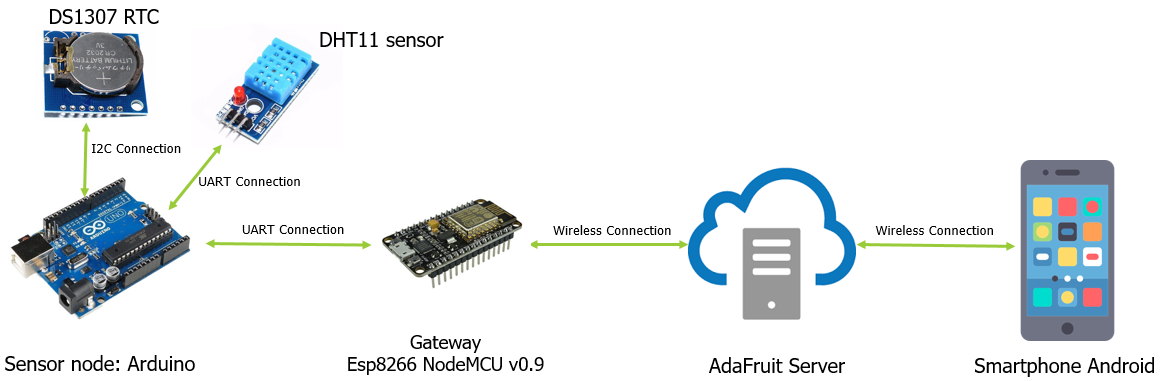
\includegraphics[width=15cm]{architechture.png}
			\caption{\textit{Architecture diagram}}
			\label{h1}
		\end{center}
	\end{figure}
	\begin{enumerate}
		\item[$\bullet$] Sensor node is used to get the value of the temperature and humidity from the environment by using DHT11 module and send to the gateway by UART Serial connection.
		\item[$\bullet$] Gateway: ESP8266 NodeMCU is used to receive the data from the sensor node (Arduino) and send to Adafruit Server through MQTT Protocol.
		\item[$\bullet$] AdaFruit.io is a free Server used to store the data that received from the gateway and send to the Smartphone based on MQTT Protocol.
		\item[$\bullet$] Smartphone Android: is used to show the data the received from the AdaFruit Server.
	\end{enumerate}
	
	\section{Sensor implementation}
	In this project, DHT11 module is used to get temperature and humidity from natural environment. Besides, a MCU used to a Sensor Node is Arduino UNO-R3. This Node's mission is receiving data from DHT11 module and real time module DS1307 RTC, packing data and sending to gateway via UART connection. Arduino always sends data packet to gateway Node each of 4 second.\\
	Data format to send data from Sensor Node to gateway is defined by JSON type like below:
	\begin{lstlisting}[language=C, caption= Json Data Format, label=test_float]
		{
			"temperature" : /*float type*/,
			"humidity" : /*float type*/,
			"date" : [
				yyyy,
				mm,
				dd
			],
			"time" : [
				hh,
				mm,
				ss
			]
		}
	\end{lstlisting}
	
	\begin{enumerate}
		\item[$\bullet$] "temperature" and "humidity" paths are data got from DHT11 module, which type of these values is float.
		\item[$\bullet$] "date" and "time" paths are real time got from DS1307 RTC module, this is the time to get data from natural environment. Server.
	\end{enumerate}
	The Source code of Arduino - sensor node is divided to 4 block: Data getting block, Real time block, Json package block and UART data sending block. \\
		\subsection{Data getting Block}
		The C source code of Data getting block is used to getting data from DHT11 via port 8, is provided below:
		\begin{lstlisting}[language=C, caption= Getting data from DHT11 sensor, label=test_float]
			............
			#include <DHT.h>
			...........
			
			//************************* DHT Sensor ************************************
			#define DHTPIN      8
			#define DHTTYPE     DHT11  
			DHT dht(DHTPIN, DHTTYPE);
			.........
			
			void setup() {
				dht.begin();
				.........
			}
			void loop() {
				// Read data from DHT11
				float temp = dht.readTemperature();
				float humi = dht.readHumidity();
				...........
			}
		\end{lstlisting}
	
		\subsection{Real time Block}
		The C source code of Real time block is used to getting real time from DS1307 RTC via I2C connection (Port A4-A5), is provided below:
		\begin{lstlisting}[language=C, caption= Getting real time from DS1307 RTC, label=test_float]
			#include <RTClib.h>
			............
			#include <time.h>
			...........
			
			//************************ RTC Sensor ************************************
			RTC_DS1307 RTC;
			.........
			
			void setup() {
				...........
				
				RTC.begin();  
				delay(500);
				// time synchronization with computer
				RTC.adjust(DateTime(__DATE__, __TIME__)); 
				...........
			}
			void loop() {
				...........
				
				// Get current time from DS1307 RTC
				DateTime now = RTC.now();
				...........
			}
		\end{lstlisting}
	
		\subsection{Json package Block}
		In this project, I used \textit{ArduinoJson.h} library version 6 to pack data format.
		The C source code of Json package block is used to packing data to Json format defined by using ArduinoJson.h lib, is provided below:
		\begin{lstlisting}[language=C, caption= Packing data to Json Type, label=test_float]
			............
			#include <ArduinoJson.h>
			...........
			
			void loop() {
				...........
				
				//********** Json Data Packages by ArduinoJson.h lib ****************
				StaticJsonDocument<256> jsonBuffer;
				JsonObject root = jsonBuffer.to<JsonObject>();
				// Add temperature-humidity path
				root["temperature"] = temp;
				root["humidity"] = humi;
				
				// Add date and time paths
				JsonArray _date = root.createNestedArray("date");
				_date.add(now.year());
				_date.add(now.month());
				_date.add(now.day());
				JsonArray _time = root.createNestedArray("time");
				_time.add(now.hour());
				_time.add(now.minute());
				_time.add(now.second());
				
				// Send Json data to Serial communication
				serializeJson(root, Serial);
				...........
			}
		\end{lstlisting}
	
		\subsection{UART data sending Block}
		The C source code of UART data sending block is used to sending data package to gateway via UART serial communication (Port 10-11), is provided below:
		\begin{lstlisting}[language=C, caption= Sending data package to gateway, label=test_float]
			............
			#include <SoftwareSerial.h>
			...........
			
			//************************ Rx - Tx ************************************
			#define RXpin       10
			#define TXpin       11
			SoftwareSerial espSerial(RXpin,TXpin);
			.........
			
			void setup() {
				...........
				
				espSerial.begin(115200);
				...........
			}
			void loop() {
				...........
				
				// Send Json data to ESP8266
				serializeJson(root, espSerial);
				...........
			}
		\end{lstlisting}
	
	\section{Gateway implementation}
	Gateway node is implemented in NodeMCU v0.9 MCU. This Node's mission is receiving data from Sensor Node (Arduino), then packing and sending to Adafruit Server.
		\subsection{UART received data}
		When the Sensor Node sent data, gateway Node received data and try to decode. Gateway Node receives data in port D1 (corresponds to RX) and sends control request via D2 (corresponds to RX). \\
		The C source code of UART data received is used to receiving data package from Sensor Node, is provided below:
		 \begin{lstlisting}[language=C, caption= Data received from Sensor Node, label=test_float]
		 	............
		 	#include <SoftwareSerial.h>
		 	...........
		 	
		 	//************************** RX-TX ***********************************************
		 	#define RXpin              D1
		 	#define TXpin              D2
		 	SoftwareSerial unoSerial(RXpin, TXpin);
		 	.........
		 	
		 	void setup() {
		 		...........
		 		
		 		unoSerial.begin(115200);
		 		...........
		 	}
		 	void loop() {
		 		...........
		 		
		 		// Get Json Data Package from Arduino
		 		DeserializationError error = deserializeJson(jsonBuffer, unoSerial);
		 		if (error){
		 			Serial.println("Fail receive data!");
		 			Serial.println(error.c_str());
		 			return;
		 		}
		 		...........
		 	}
		 \end{lstlisting}
		 \textit{deserializeJson()} is a function of \textit{AndroidJson.h} library, it used to get Json data package from serial communication.
		 \subsection{Data uploading process}
		 After the sensory data is received by the gateway, the data package will be uploaded to Adafruit Server by using MQTT protocol. Before data packet was sent, it is format to a string with Json format, is implemented below:
		 \begin{lstlisting}[language=C, caption= Json Data Format, label=test_float]
		 	{
		 		"temperature" : /*float type*/,
		 		"humidity" : /*float type*/,
		 		"date" : "yyyy-mm-ddThh:mm:ss"
		 	}
		 \end{lstlisting}
		 Compared to the data format sent from the node, the packet sent to the server is changed the format of "date" to the standard date type of Json format. This will help clients is easier to decode data packet. \\
		 The C source code of UART data received is used to receiving data package from Sensor Node, is provided below:
		 \begin{lstlisting}[language=C, caption= MQTT sending data, label=test_float]
		 	............
		 	#include "Adafruit_MQTT.h"                    
		 	#include "Adafruit_MQTT_Client.h"                 
		 	
		 	#include <ESP8266WiFi.h>
		 	...........
		 	
		 	//*********** Wifi via Access Point *********
		 	#define WIFI_SSID       "Muoi Vinh"    //"6-No-2-Hope-3"
		 	#define WIFI_PASSWORD   "0988258072"    //"01072000"
		 	
		 	// Create an ESP8266 WiFiClient class to connect to the MQTT server.
		 	WiFiClient client;
		 	
		 	//************ Adafruit.io Setup **********
		 	#define AIO_SERVER      "io.adafruit.com"
		 	#define AIO_SERVERPORT  1883                               
		 	#define AIO_USERNAME    "vitran"                            
		 	#define AIO_KEY         "aio_kMjj660iSchQ5gVRBDF39N9COyEh"           
		 	
		 	//************** Setup MQTT client class *****************
		 	// Passing in the WiFi client and MQTT server and login details.
		 	Adafruit_MQTT_Client mqtt(&client, AIO_SERVER, AIO_SERVERPORT, AIO_USERNAME, AIO_KEY);
		 	
		 	//************ Feeds ****************
		 	Adafruit_MQTT_Publish motion = Adafruit_MQTT_Publish(&mqtt, AIO_USERNAME "/feeds/temperature");
		 	.........
		 	
		 	void setup() {
		 		...........
		 		
		 		connectWifi();
		 		...........
		 	}
		 	void loop() {
		 		...........
		 		
		 		if(!motion.publish(val.c_str()))
		 		Serial.println("Send data Failed!");
		 		else
		 		Serial.println("Data sent!");
		 		
		 		// Ping Adafruit.IO to keep the MQTT connection alive
		 		if(! mqtt.ping()) {
		 			mqtt.disconnect();
		 		}                
		 		...........
		 	}
	 		//*************** WiFi Connection *************
	 		void connectWifi()
	 		{   
	 			// If already connected to WiFi, return to loop
	 			if (WiFi.status() == WL_CONNECTED){ return; }        
	 			
	 			// Start a WiFi connection and enter SSID and Password   
	 			WiFi.begin(WIFI_SSID, WIFI_PASSWORD);   
	 			
	 			// While waiting on connection to start display "..."                   
	 			while (WiFi.status() != WL_CONNECTED) {     
	 				delay(500);
	 				Serial.print(".");                  
	 			} 
	 			Serial.println("Connected");    
	 			
	 			// Run Procedure to connect to Adafruit IO MQTT                        
	 			MQTT_connect();                               
	 		}
	 		
	 		//************ MQTT Connect - Adafruit IO ***********
	 		void MQTT_connect() 
	 		{
	 			int8_t ret;
	 			
	 			// Stop if already connected to Adafruit
	 			if (mqtt.connected()) { return; }                       
	 			Serial.println("Connecting to MQTT... ");
	 			
	 			mqtt.disconnect();
	 			
	 			// Connect to Adafruit, will return 0 if connected
	 			while ((ret = mqtt.connect()) != 0) {                   
	 				Serial.println(mqtt.connectErrorString(ret));
	 				Serial.println("Retrying MQTT...");
	 				mqtt.disconnect();
	 				delay(5000);                                       // wait 5 seconds
	 			}
	 			Serial.println("MQTT Connected!");  
	 		}
		 \end{lstlisting}
		 Data sent to MQTT server is character type, so we should change data format to string and use \textit{c$\_$str()} to change to character type.
		\begin{figure}[h!]
			\begin{center}
				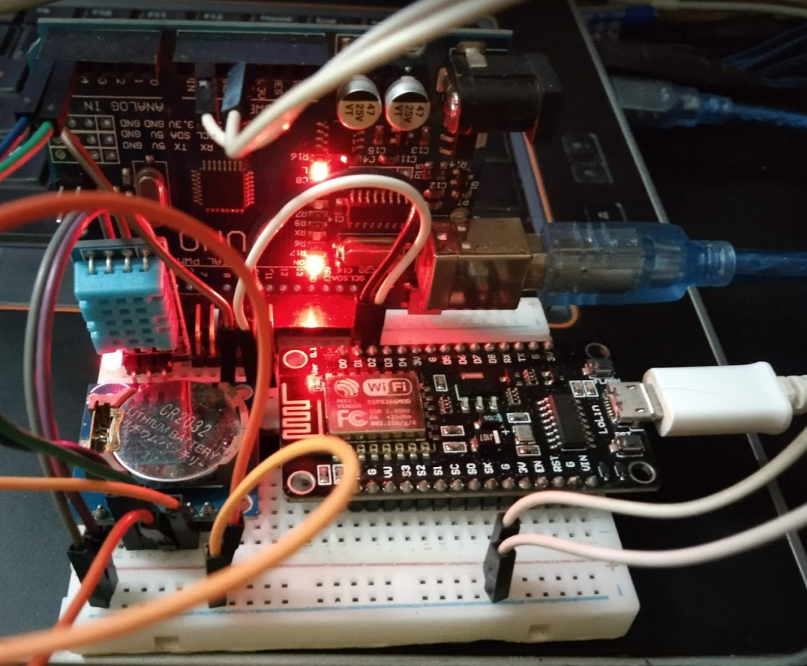
\includegraphics[width=10cm]{node.png}
				\caption{\textit{Sensor Node and Gateway Node}}
			\end{center}
		\end{figure}
	\section{Server configuration}
	In this Project, as a description above, we use Adafruit.io server to serve data sent from Sensor Nodes. \\
	Adafruit.io is a system that makes data useful. Our focus is on ease of use, and allowing simple data connections with little programming required. It includes client libraries that wrap our REST and MQTT APIs. So, it is very suitable for this Project. \\
	Besides, we can use other web server like Thingspeak,... \\
	 \begin{figure}[h!]
	 	\begin{center}
	 		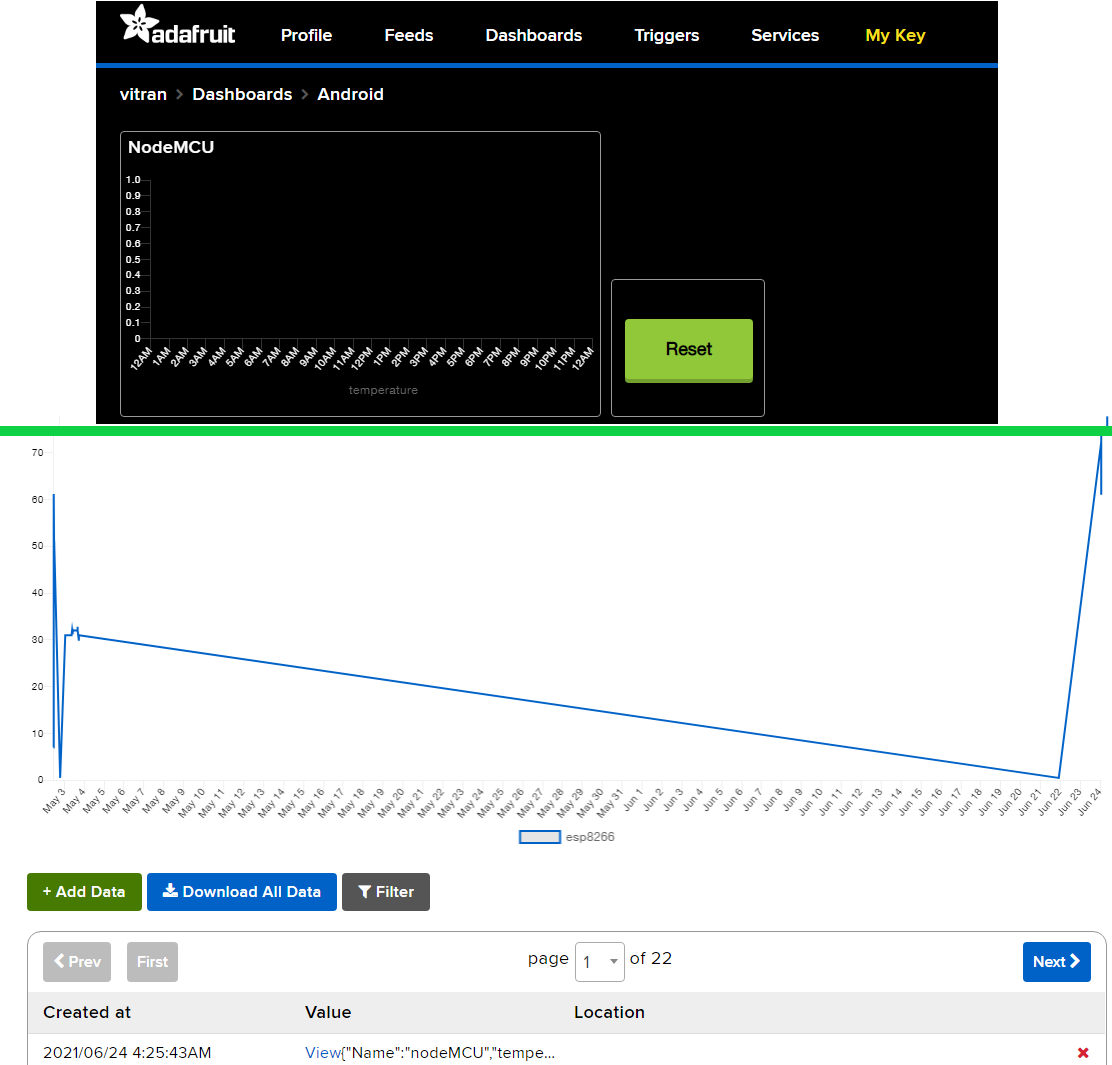
\includegraphics[width=10cm]{adafruit.png}
	 		\caption{\textit{Adafruit MQTT Server UI}}
	 	\end{center}
	 \end{figure}
	A public server URL of this project is \url{"https://io.adafruit.com/vitran/feeds/temperature"}.
	\section{Monitoring application}
	After all, we build an Android app to get data from Adafruit server and present in the app UI as graphs and lastest updated data.
	\begin{figure}[h!]
		\begin{center}
			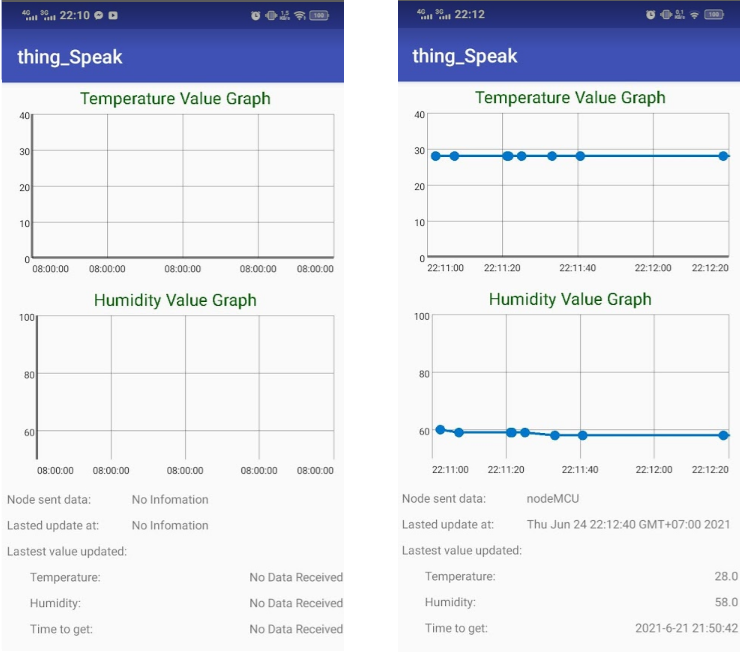
\includegraphics[width=15cm]{app.png}
			\caption{\textit{Android app UI}}
		\end{center}
	\end{figure}
	\\ 
	This app includes temperature and humidity graph and parameter path. \\
	In parameter path, we can see name of Node sent data, the last time data was subscribed from server and and parts of the data after being decoded. 
	
	\newpage
	\section{Conclusion}
	In conclusion, this project has realized serial communication between devices and wireless communication between devices and MQTT server.\\
	In the future, this project can be extended with multiple Nodes and the android app can send commands to control the specific peripherals of each node.\\
	You can watch demo video at \\ \url{https://drive.google.com/file/d/1gWIa9NhSV-E2T5hbH-LKRj745DvZ4ytM/view?usp=sharing}
	
	%%%%%%%%%%%%%%%%%%%%%%%%%%%%%%%%%
	\newpage
	\addcontentsline{toc}{section}{Reference}
	\begin{thebibliography}{99999}	
		\bibitem[Web]{1}{Arduino,} {\url{https://www.arduino.cc/}}
		\bibitem[Web]{1}{ArduinoJson v6,} {\url{https://arduinojson.org/v6/doc/}}
		\bibitem[Web]{1}{Android Graph,} {\url{https://www.geeksforgeeks.org/line-graph-view-in-android-with-example/}}
		
	\end{thebibliography}
\end{document}
\end{document}